\newpage
\section{Experimentos y Análisis de Resultados}
\label{sec:experimentos}

\subsection{Configuración Experimental y Parámetros}

Para evitar redundancias, se remite al Punto \ref{sec:formulacion} para la definición formal del problema, los conjuntos de datos (IBEX 35, S\&P 100 y S\&P 500) y las restricciones sobre las posiciones de los activos. A continuación se especifican únicamente los detalles experimentales necesarios para la reproducibilidad y la comparación empírica.

\subsubsection*{Condiciones de ejecución}

\begin{itemize}
    \item \textbf{Ejecuciones independientes:} 50 por algoritmo y mercado. Semilla base $seed=42$, incrementada secuencialmente ($42+i$).
    \item \textbf{Criterio de parada:} máximo de 10\,000 evaluaciones de la función objetivo para todas las técnicas, garantizando comparabilidad.
    \item \textbf{Neutralidad de datos:} los mismos historiales y particiones temporales se utilizan para todas las ejecuciones y métodos.
\end{itemize}

\subsubsection*{Parámetros de los algoritmos poblacionales}

Los parámetros experimentales de los algoritmos evolutivos se fijan como sigue (valores aplicados de forma homogénea salvo indicación contraria):

\begin{description}
    \item[Tamaño de la población:] $|P| = 100$.
    \item[Selección:] torneo de tamaño $k=3$.
    \item[Cruce:] $P_c = 0.8$ para AGG; $P_c = 1.0$ para AGE. Para BLX-$\alpha$, $\alpha = 0.3$.
    \item[Mutación:] $P_m = 0.1$ a nivel de individuo. La mutación implementada es de tipo transferencia suave (traslado de capital entre genes), con magnitud de transferencia fijada en 15\% cuando aplica.
\end{description}

\subsubsection*{Parámetros de la búsqueda local (algoritmos meméticos)}

La hibridación con Búsqueda Local se parametriza para equilibrar intensidad y costo computacional:

\begin{itemize}
    \item \textbf{Frecuencia:} cada 10 generaciones.
    \item \textbf{Aplicación:} \textbf{AM-Rand} aplica BL con probabilidad $P_{LS}=0.1$ por cromosoma; \textbf{AM-Best} aplica BL sólo al 10\% superior.
    \item \textbf{Intensidad:} máximo 100 evaluaciones por invocación de BL; radio de transferencia entre empresas reducido al 15\% para minimizar perturbaciones radicales.
\end{itemize}

Estas elecciones persiguen asegurar comparabilidad entre métodos y mantener el coste computacional dentro de límites razonables para las series temporales utilizadas.

\subsection{Resultados Numéricos Globales y Boxplots}

En esta sección se resumen los resultados globales obtenidos a partir de la ejecución del experimento, mostrando únicamente los algoritmos exigidos en el guion: Greedy, Random, BL, AGG-Arit, AGG-BLX, AGE-Arit, AGE-BLX, AM-All, AM-Rand y AM-Best.

\begin{table}[H]
\centering
\caption{Resultados numéricos globales -- IBEX 35}
\label{tab:global-ibex35}
\resizebox{\textwidth}{!}{%
\begin{tabular}{lccccc}
\hline
Algoritmo & Fitness(2015--2024) & Fitness(2025) & Beneficio & Evaluaciones & Tiempo (s) \\
\hline
Greedy   & -4.794 & -3.227 & -0.033 & 1     & 0.000 \\
Random   & -4.911 & -3.305 &  0.052 & 10000 & 0.024 \\
BL       & -4.614 & -3.116 &  0.021 & 1078  & 0.001 \\
AGG-Arit & -4.663 & -3.142 &  0.042 & 10000 & 0.009 \\
AGG-BLX  & -4.496 & -3.091 &  0.036 & 10000 & 0.010 \\
AGE-Arit & -4.587 & -3.119 &  0.043 & 10000 & 0.010 \\
AGE-BLX  & -4.499 & -3.097 &  0.033 & 10000 & 0.011 \\
AM-All   & -4.591 & -3.118 &  0.036 & 10000 & 0.008 \\
AM-Rand  & -4.490 & -3.084 &  0.033 & 10000 & 0.009 \\
AM-Best  & -4.490 & -3.083 &  0.033 & 10000 & 0.009 \\
\hline
\end{tabular}
}
\end{table}

\begin{table}[H]
\centering
\caption{Resultados numéricos globales -- S\&P 100}
\label{tab:global-sp100}
\resizebox{\textwidth}{!}{%
\begin{tabular}{lccccc}
\hline
Algoritmo & Fitness(2015--2024) & Fitness(2025) & Beneficio & Evaluaciones & Tiempo (s) \\
\hline
Greedy   & -3.305 & -3.791 & 0.100 & 1     & 0.000 \\
Random   & -3.400 & -4.080 & 0.079 & 10000 & 0.098 \\
BL       & -3.116 & -3.890 & 0.097 & 4351  & 0.033 \\
AGG-Arit & -3.120 & -3.845 & 0.083 & 10000 & 0.071 \\
AGG-BLX  & -2.879 & -3.721 & 0.096 & 10000 & 0.075 \\
AGE-Arit & -3.157 & -3.872 & 0.082 & 10000 & 0.071 \\
AGE-BLX  & -2.937 & -3.744 & 0.094 & 10000 & 0.075 \\
AM-All   & -3.110 & -3.830 & 0.085 & 10000 & 0.073 \\
AM-Rand  & -2.822 & -3.735 & 0.099 & 10000 & 0.074 \\
AM-Best  & -2.814 & -3.740 & 0.102 & 10000 & 0.074 \\
\hline
\end{tabular}
}
\end{table}

\begin{table}[H]
\centering
\caption{Resultados numéricos globales -- S\&P 500}
\label{tab:global-sp500}
\resizebox{\textwidth}{!}{%
\begin{tabular}{lccccc}
\hline
Algoritmo & Fitness(2015--2024) & Fitness(2025) & Beneficio & Evaluaciones & Tiempo (s) \\
\hline
Greedy   & -3.370 & -3.909 & 0.024 & 1     & 0.000 \\
Random   & -3.648 & -4.364 & 0.019 & 10000 & 1.851 \\
BL       & -3.428 & -4.330 & 0.004 & 9645  & 1.526 \\
AGG-Arit & -2.961 & -3.958 & 0.018 & 10000 & 1.504 \\
AGG-BLX  & -2.791 & -3.893 & 0.023 & 10000 & 1.490 \\
AGE-Arit & -3.176 & -4.073 & 0.018 & 10000 & 1.478 \\
AGE-BLX  & -3.012 & -3.984 & 0.023 & 10000 & 1.483 \\
AM-All   & -3.204 & -4.102 & 0.015 & 10000 & 1.573 \\
AM-Rand  & -2.738 & -3.907 & 0.017 & 10000 & 1.537 \\
AM-Best  & -2.731 & -3.905 & 0.017 & 10000 & 1.538 \\
\hline
\end{tabular}
}
\end{table}

A continuación se presentan los boxplots correspondientes a cada mercado para su posterior análisis:

% Imágenes PR2 obligatorios por mercado
\begin{figure}[H]
\centering
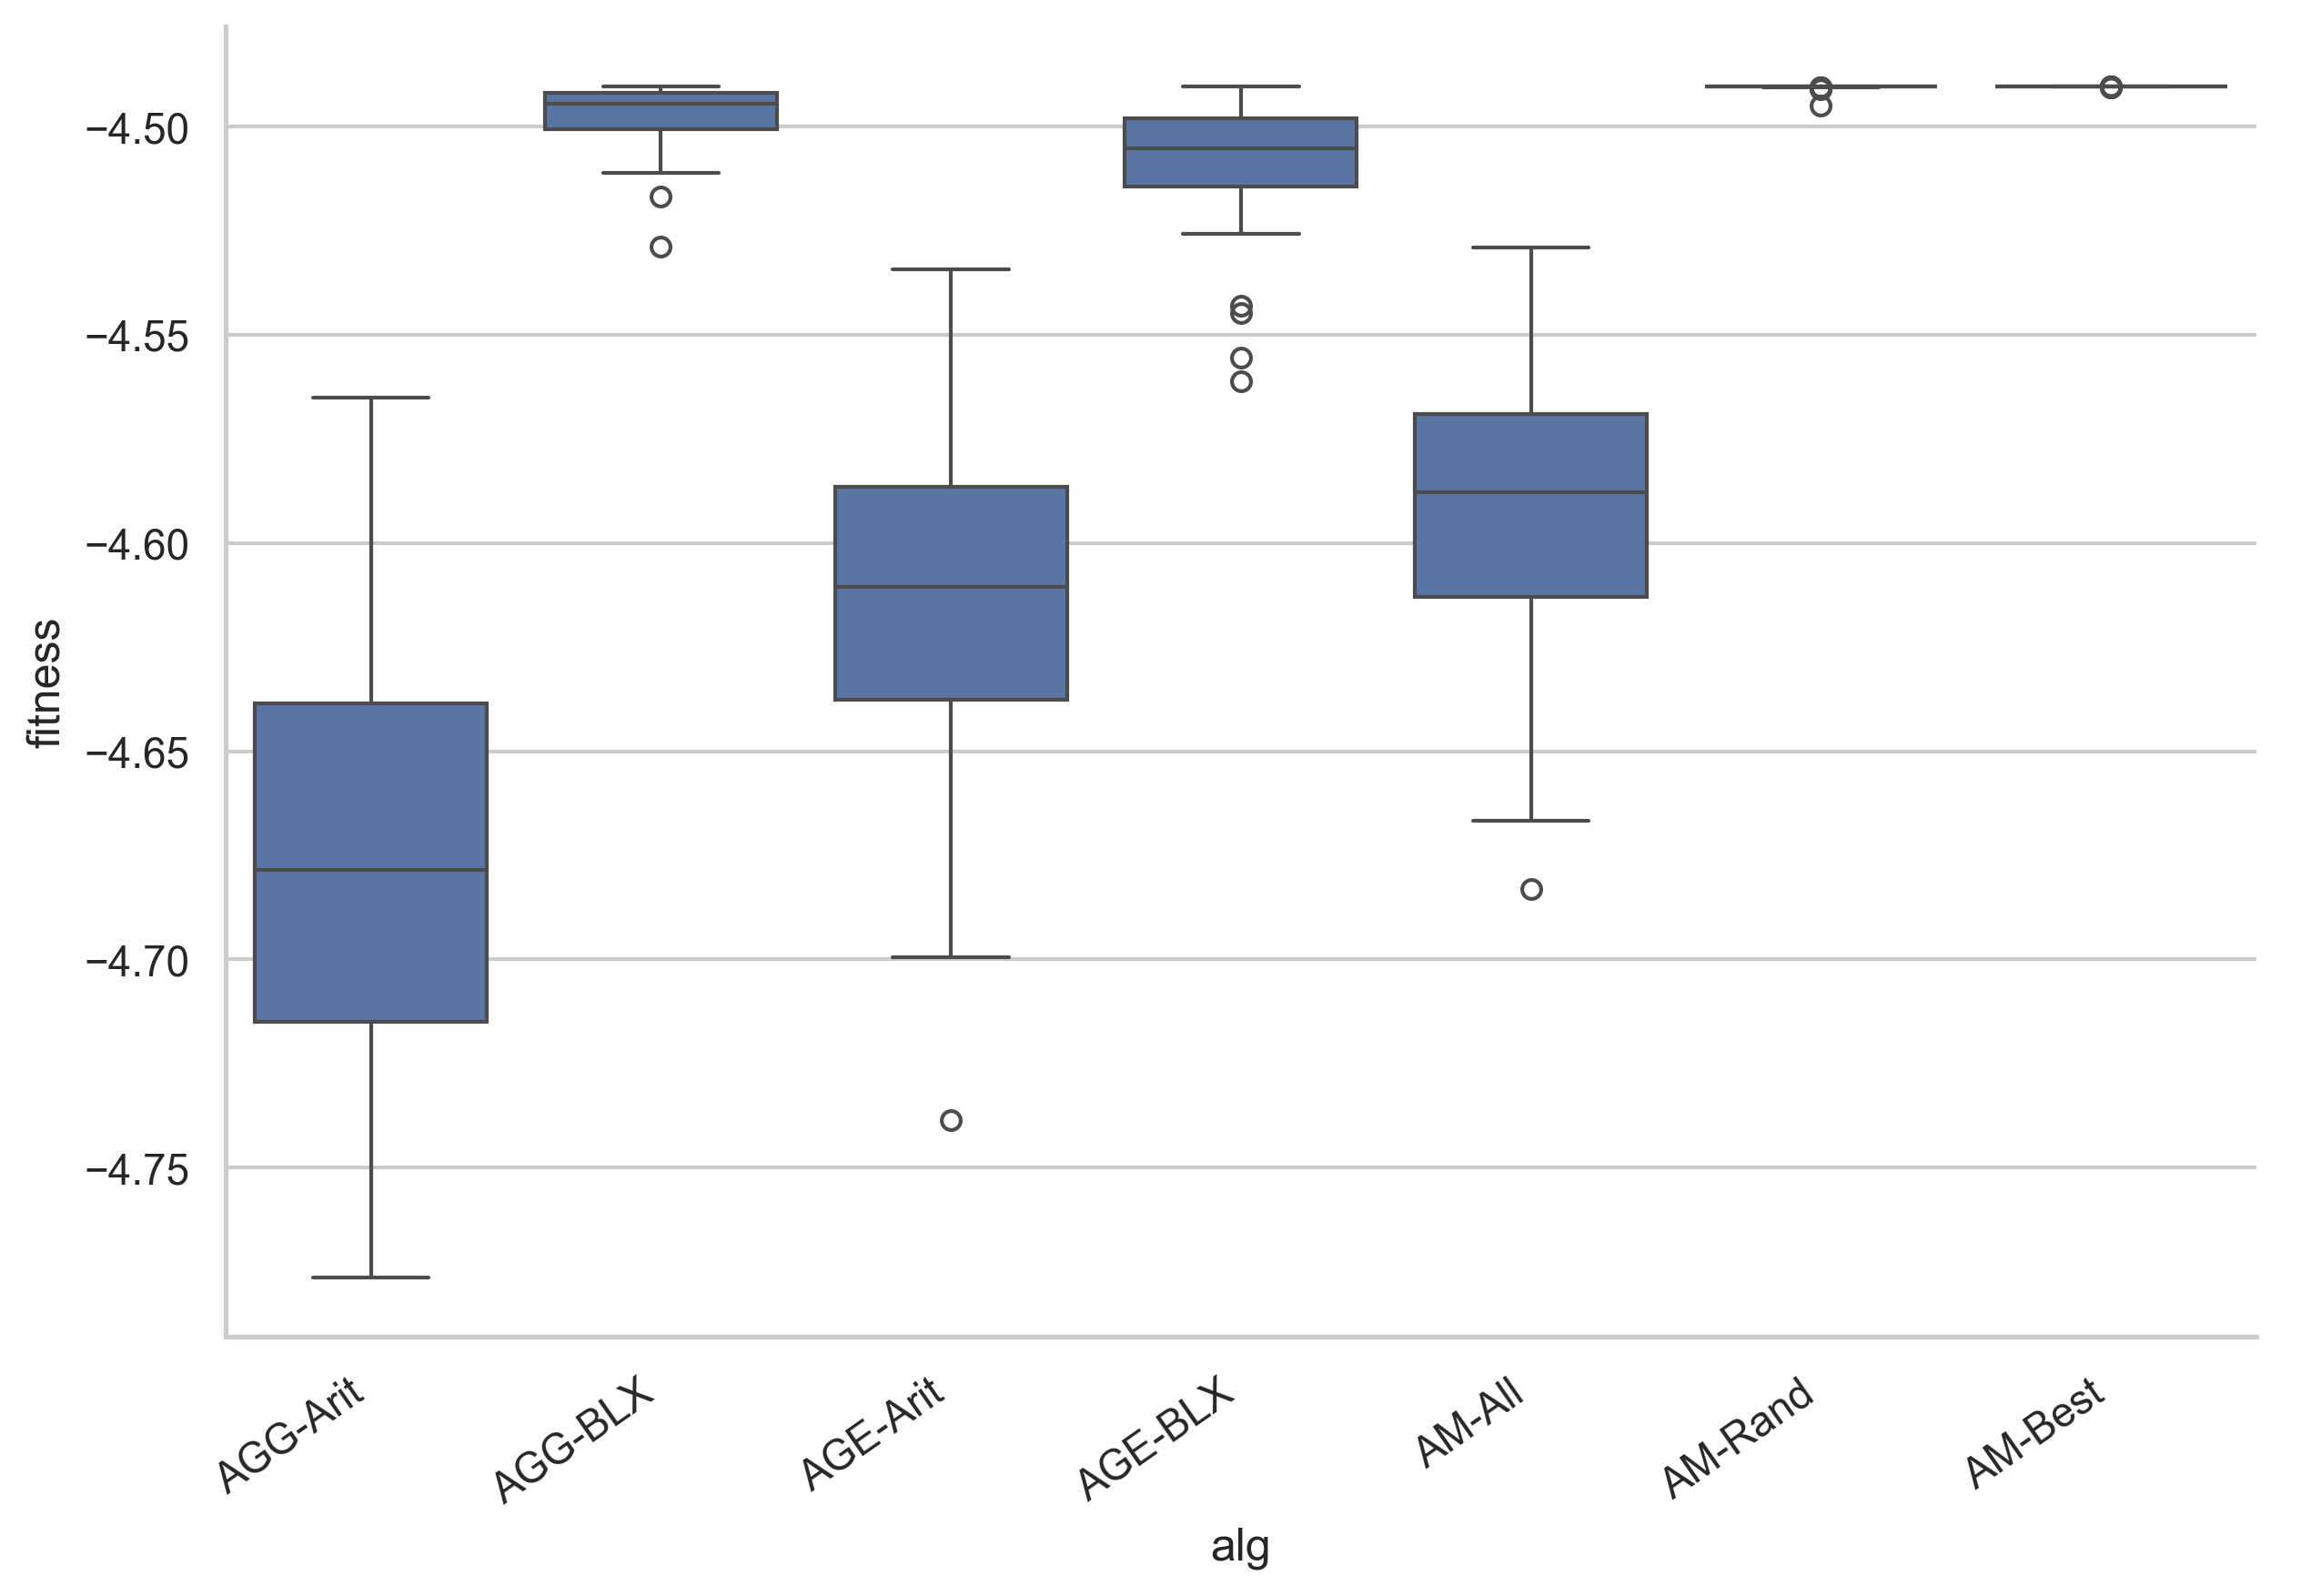
\includegraphics[width=0.8\textwidth]{figuras/IBEX_35_RESULTS_pr2_obligatorios.png}
\caption{Boxplots algoritmos práctica 2 -- IBEX 35.}
\label{fig:pr2-obligatorios-ibex}
\end{figure}

\begin{figure}[H]
\centering
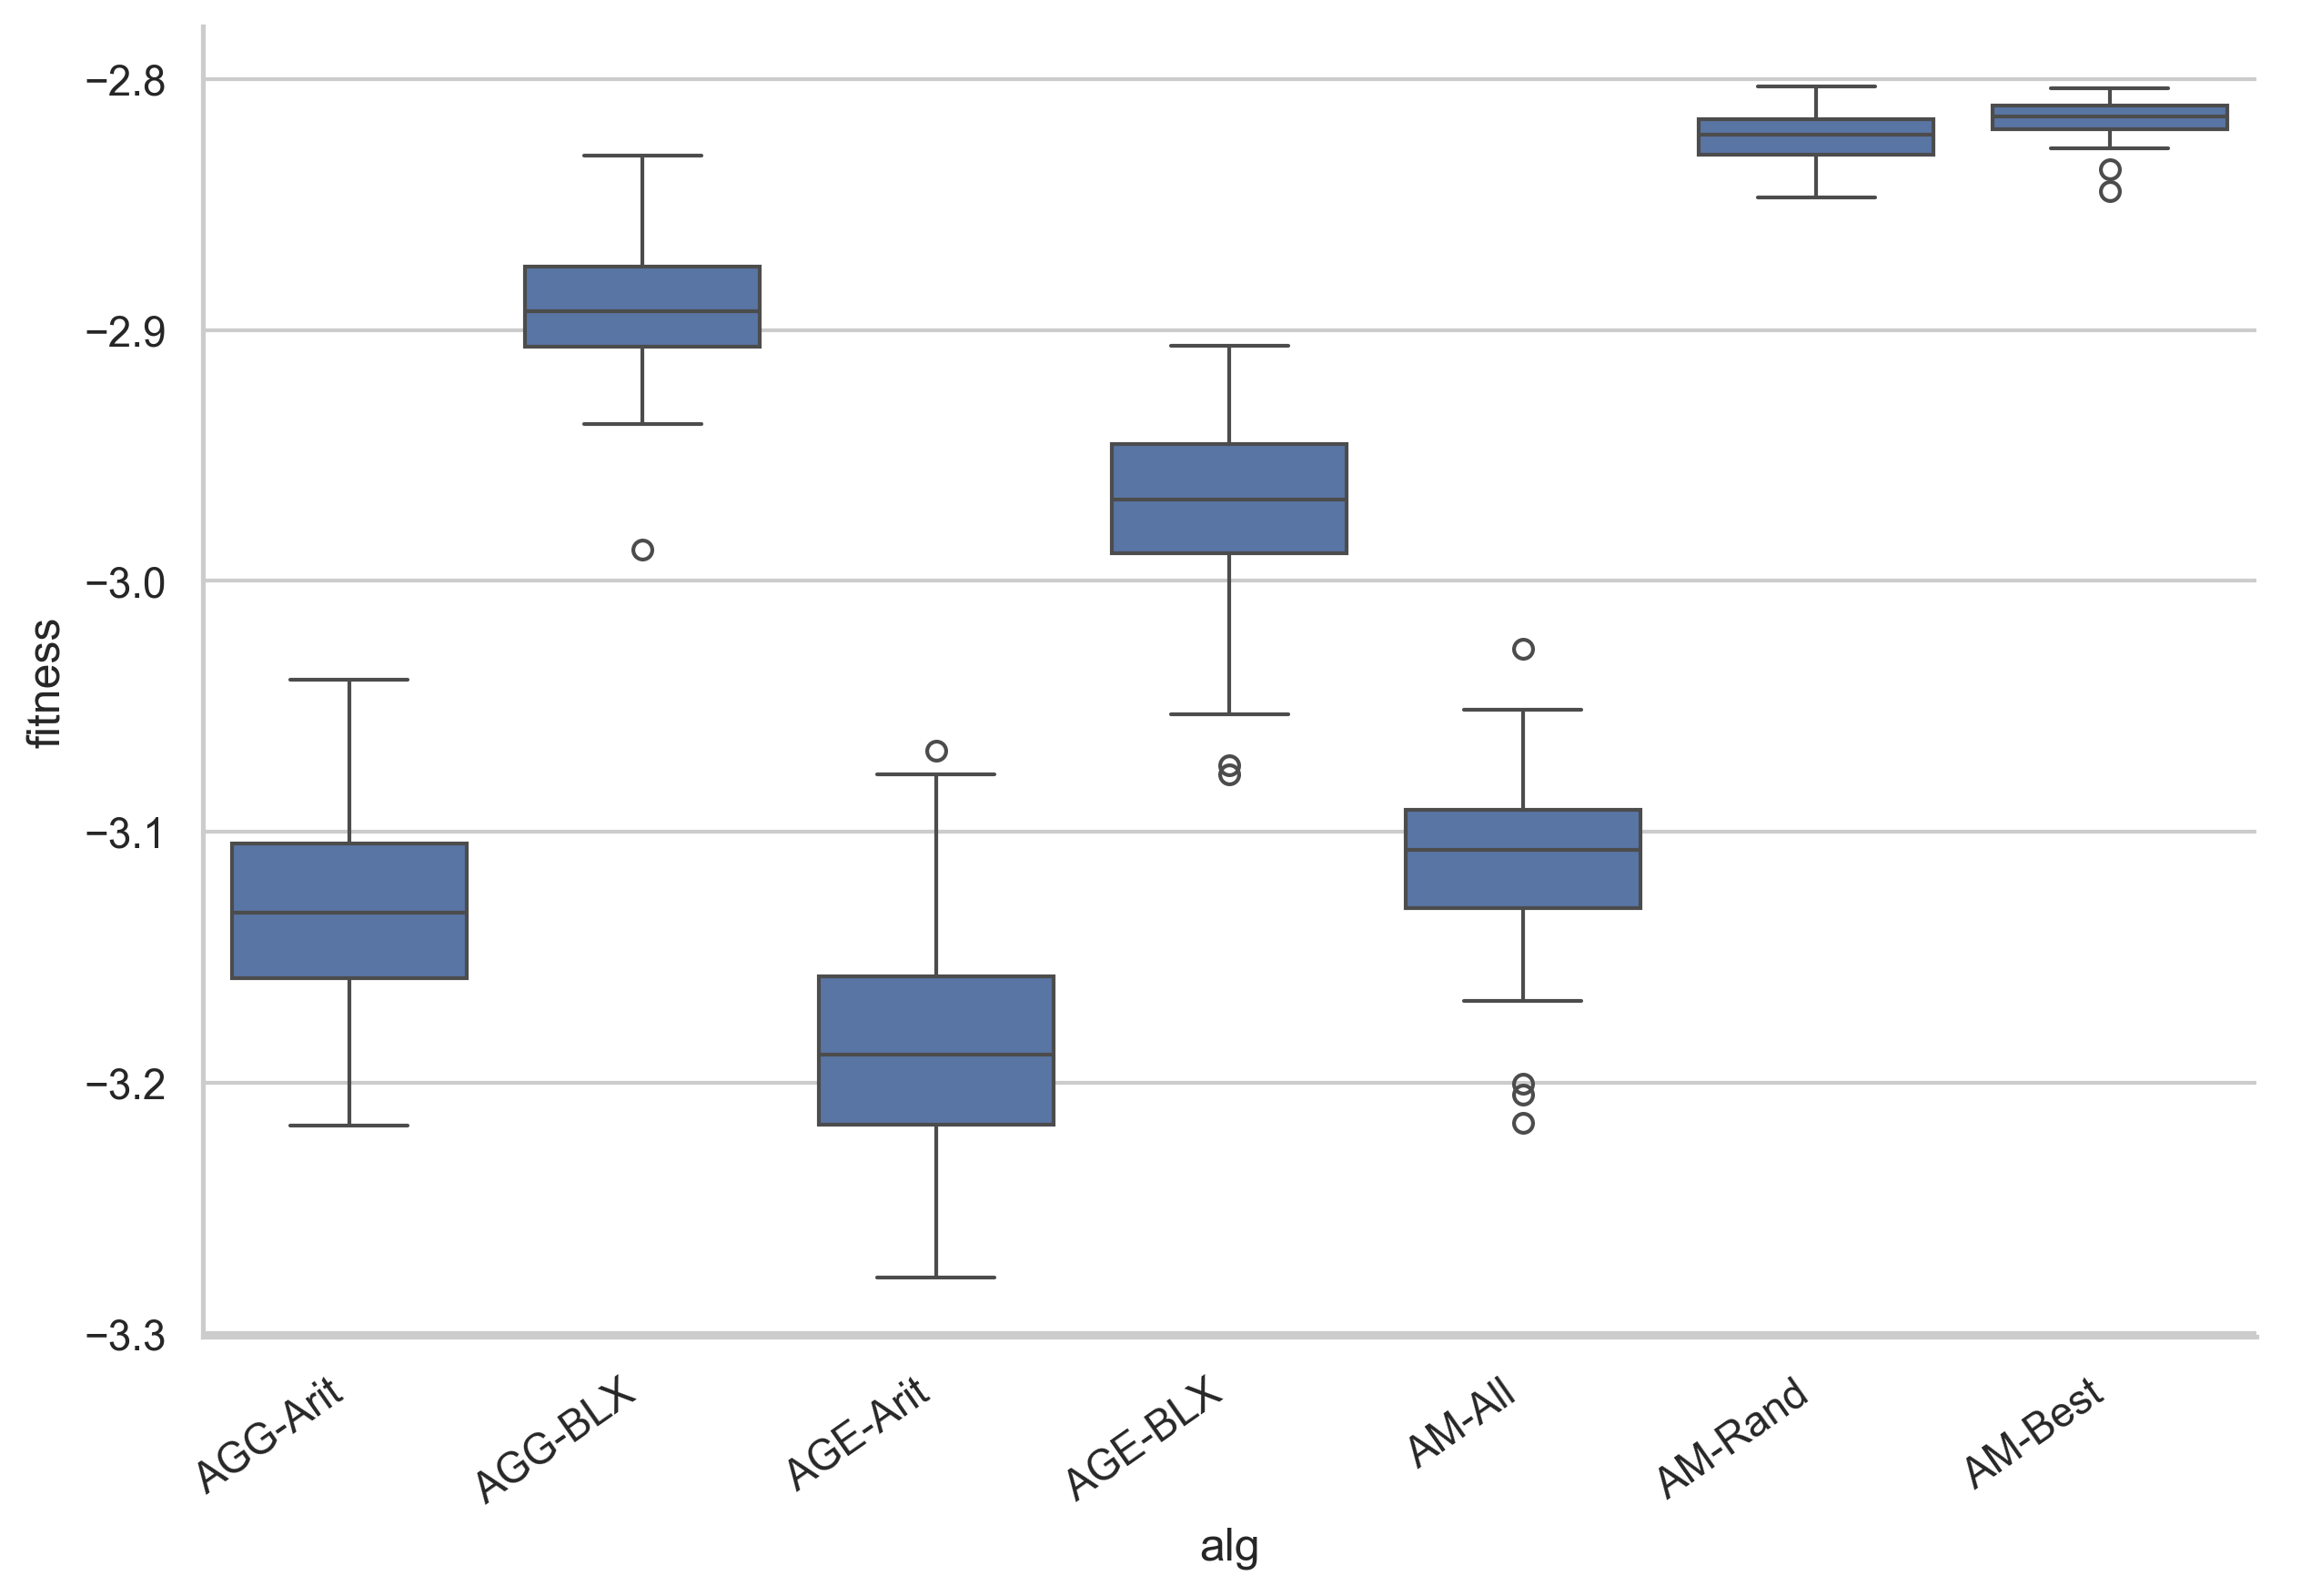
\includegraphics[width=0.8\textwidth]{figuras/S&P_100_RESULTS_pr2_obligatorios.png}
\caption{Boxplots algoritmos práctica 2 -- S\&P 100.}
\label{fig:pr2-obligatorios-sp100}
\end{figure}

\begin{figure}[H]
\centering
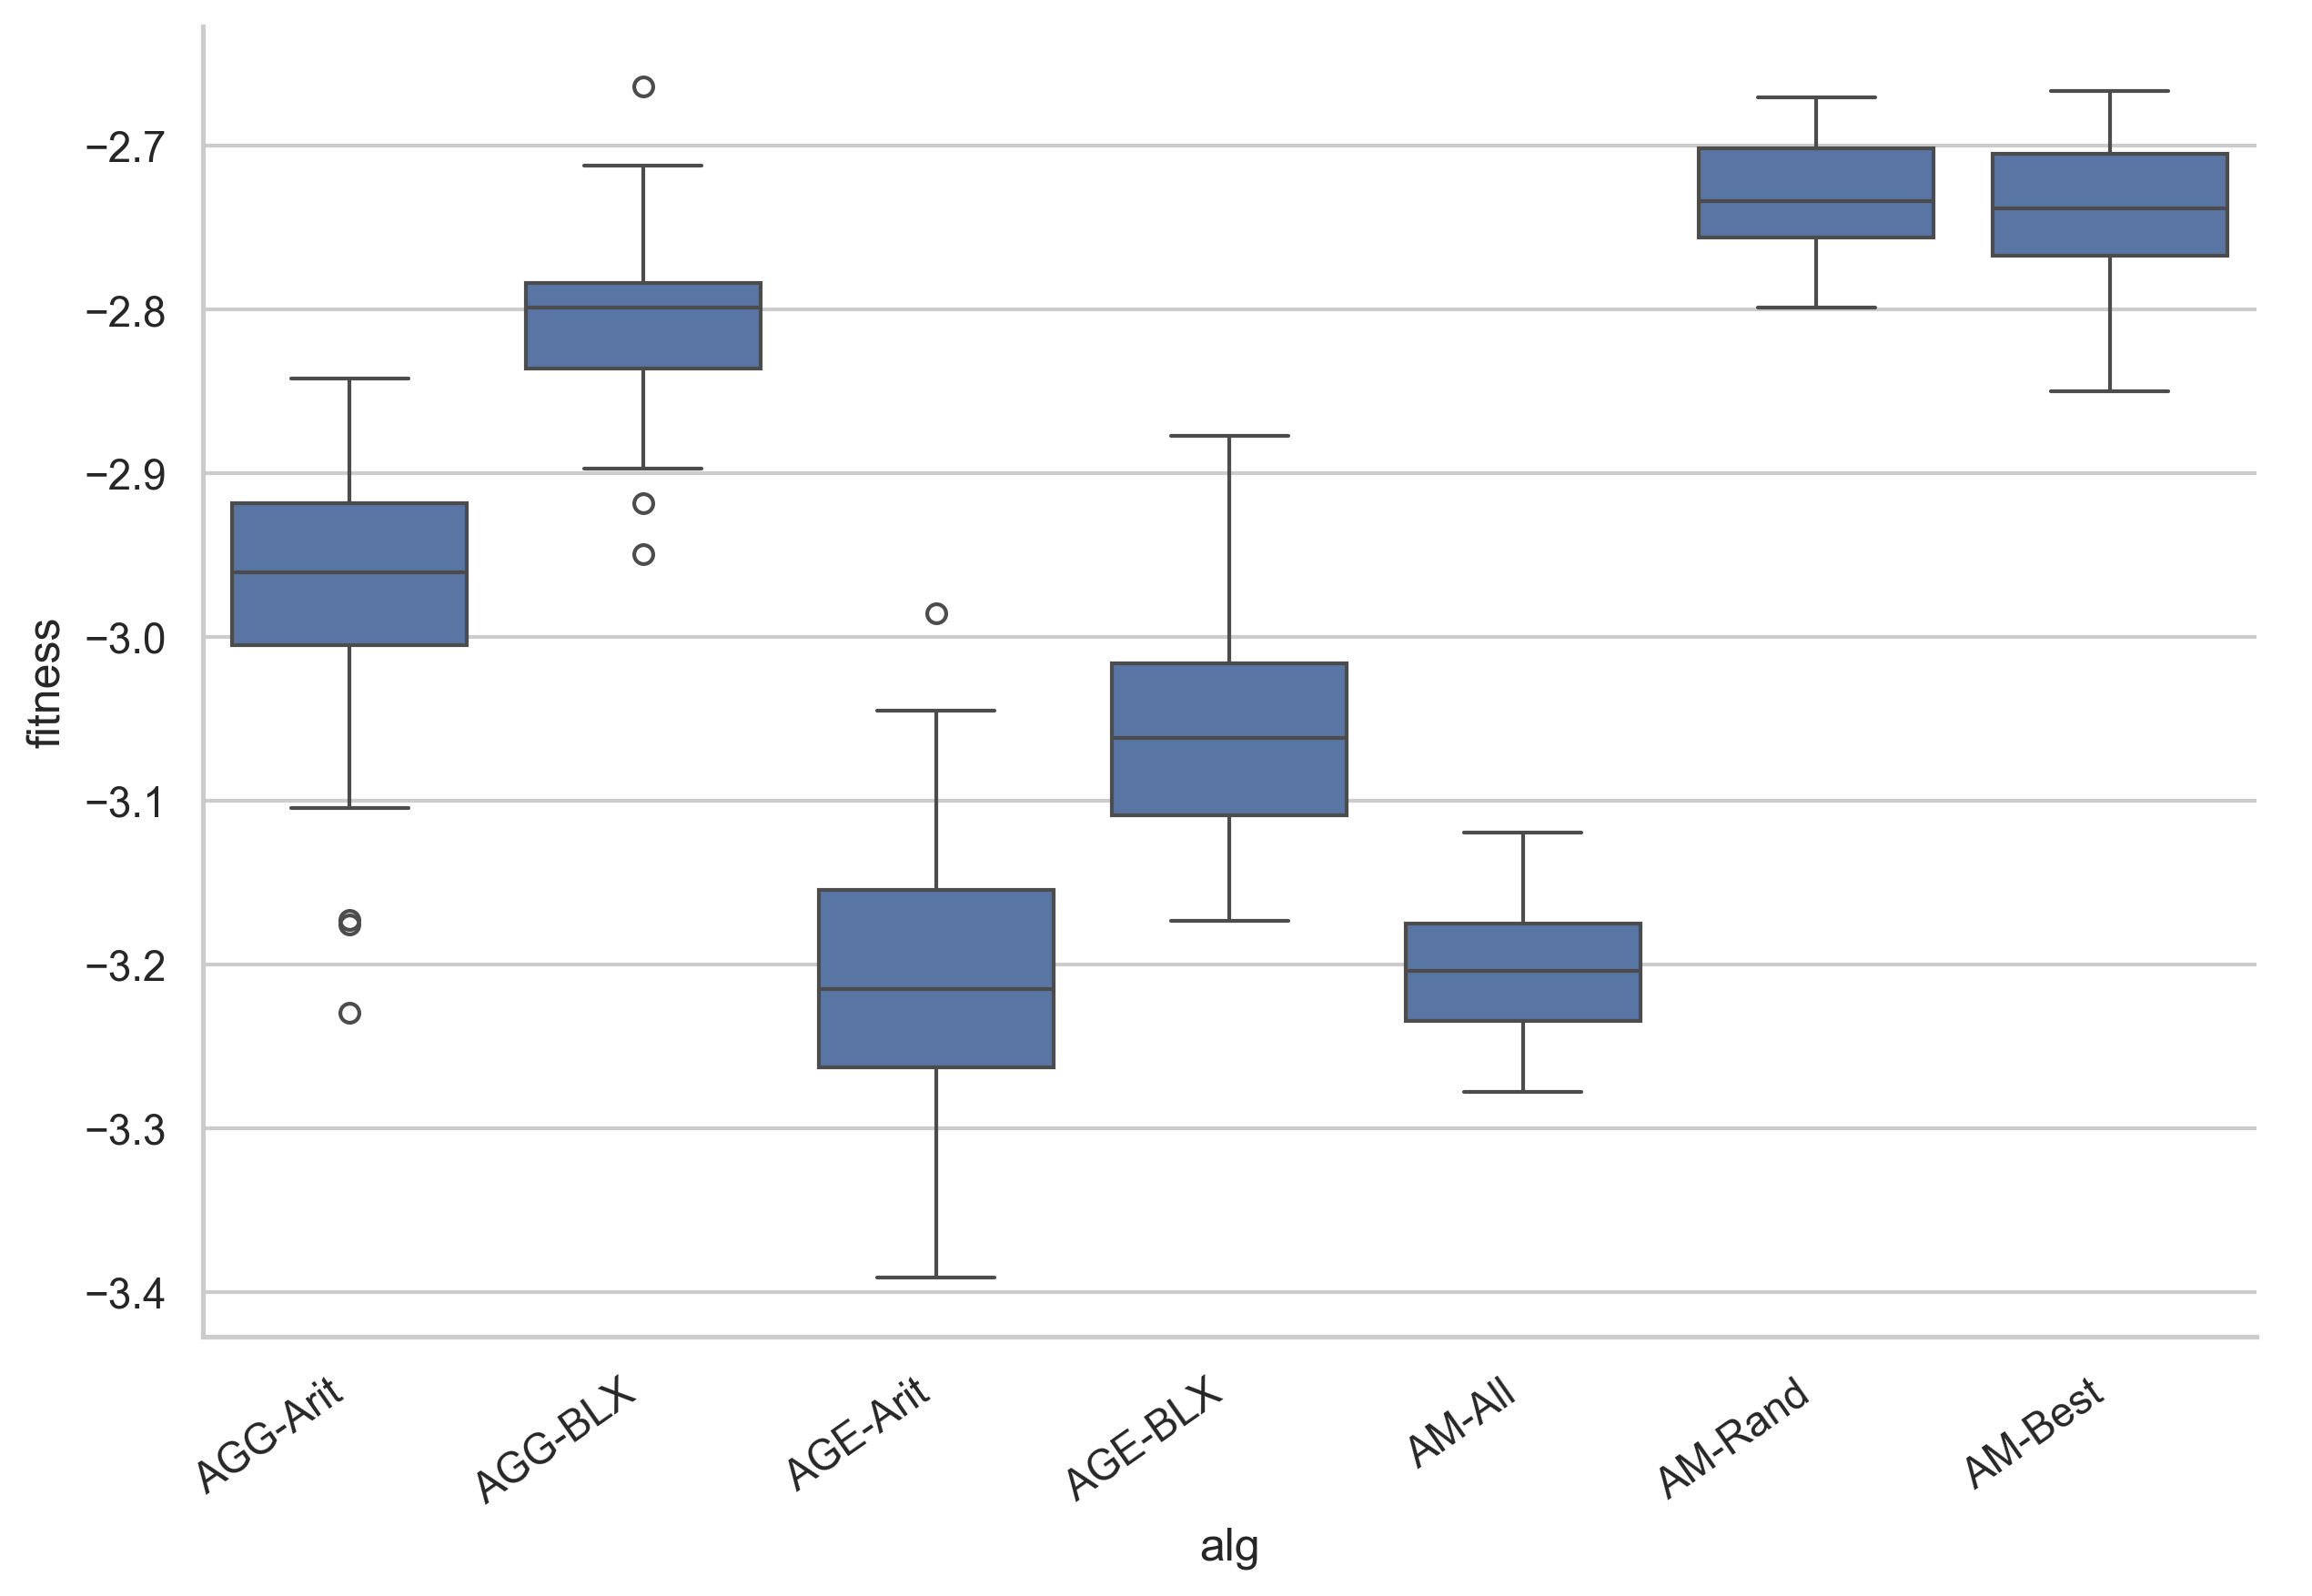
\includegraphics[width=0.8\textwidth]{figuras/S&P_500_RESULTS_pr2_obligatorios.png}
\caption{Boxplots algoritmos práctica 2 -- S\&P 500.}
\label{fig:pr2-obligatorios-sp500}
\end{figure}


\subsection{Análisis de los Algoritmos Genéticos}

En este apartado se comparan las cuatro variantes genéticas puras ---AGG-Arit, AGG-BLX, AGE-Arit y AGE-BLX--- atendiendo a tres ejes: calidad media de las soluciones (fitness en el periodo de 2015--2024), dispersión entre ejecuciones y presencia de valores atípicos. La discusión se apoya en los boxplots de las Figuras~\ref{fig:pr2-obligatorios-ibex},~\ref{fig:pr2-obligatorios-sp100} y~\ref{fig:pr2-obligatorios-sp500}, así como en las tablas globales previamente presentadas, y se articula desde una perspectiva comparativa y porcentual, sin limitarse a una mera lectura de cifras.

\subsubsection*{Efecto del operador de cruce: Aritmético frente a BLX-$\alpha$}

El resultado más contundente y sistemático que arrojan los tres mercados es la superioridad del cruce BLX-$\alpha$ sobre el cruce aritmético, independientemente del modelo evolutivo empleado. En el IBEX~35, las variantes BLX mejoran a sus homólogas aritméticas en torno a un 3--4\,\% en fitness medio; en el S\&P~100 la mejora se amplía hasta aproximadamente un 7--8\,\%, y en el S\&P~500 alcanza valores cercanos al 5--6\,\%. Este patrón creciente con la dimensionalidad del mercado no resulta casual: el cruce BLX-$\alpha$, al expandir el intervalo de exploración un factor $\alpha\!\cdot\!I$ por encima y por debajo del rango definido por los padres, introduce diversidad genética adicional que resulta tanto más valiosa cuanto mayor es el espacio de búsqueda. El cruce aritmético, por contra, se limita a interpolar linealmente entre los valores parentales, lo que restringe las nuevas soluciones al interior del hipervolumen definido por la población actual y favorece una convergencia prematura hacia zonas que pueden no contener el óptimo global.

\subsubsection*{Modelo generacional frente a estacionario}

La comparación entre el modelo generacional (AGG) y el estacionario (AGE) resulta algo más matizada. En el IBEX~35, ambos modelos con cruce BLX rinden de forma prácticamente indistinguible ---sus medianas difieren muy poco---, lo cual indica que, para un mercado de dimensión reducida, la presión selectiva adicional del AGE no aporta una ventaja significativa. Sin embargo, en los mercados de mayor dimensión la tendencia se invierte: en el S\&P~100, el AGG-BLX supera al AGE-BLX en torno a un 2\,\%, y en el S\&P~500 esta diferencia se amplía hasta cerca del 7\,\%. De forma análoga, AGG-Arit supera a AGE-Arit en el S\&P~500 por un margen cercano al 7\,\%, mientras que en el S\&P~100 ambas variantes aritméticas quedan muy próximas.

Esta degradación relativa del modelo estacionario cuando aumenta la dimensión se explica por su inherente presión selectiva: el AGE reemplaza en cada iteración únicamente a los dos peores cromosomas de la población, lo que provoca una convergencia muy rápida de la población hacia los mejores individuos. En mercados con pocas empresas (IBEX~35, 35 activos), esa convergencia rápida resulta compatible con una exploración razonable del espacio; pero a medida que la dimensión crece (100 o 500 activos), la pérdida prematura de diversidad impide al AGE descubrir regiones prometedoras que un AGG, al renovar la población completa en cada generación, sí logra alcanzar.

\subsubsection*{Variabilidad y robustez de las soluciones}

Los boxplots revelan diferencias muy notorias en la dispersión de las 50 ejecuciones. Las variantes con cruce aritmético exhiben, de forma consistente, las cajas más amplias y los bigotes más extendidos:

\begin{itemize}
    \item En el IBEX~35 (Figura~\ref{fig:pr2-obligatorios-ibex}), AGG-Arit presenta la mayor caja de todas las variantes genéticas, con un rango intercuartílico que abarca aproximadamente el doble que el de AGG-BLX. AGE-Arit, si bien algo más concentrado que AGG-Arit, muestra también una dispersión considerablemente mayor que las variantes BLX.
    \item En el S\&P~100 (Figura~\ref{fig:pr2-obligatorios-sp100}), AGE-Arit es la variante con mayor amplitud de caja y los bigotes más largos. AGG-Arit le sigue en variabilidad, mientras que AGG-BLX concentra sus resultados en una banda estrecha.
    \item En el S\&P~500 (Figura~\ref{fig:pr2-obligatorios-sp500}), el caso más llamativo es nuevamente AGE-Arit, cuyo bigote inferior se extiende mucho más que el de cualquier otra variante ---prácticamente el doble del rango de AGG-BLX---, reflejando una alta inestabilidad entre ejecuciones.
\end{itemize}

Esta mayor variabilidad del cruce aritmético se explica porque, al interpolar exclusivamente dentro del rango parental, el resultado depende en exceso de la diversidad inicial de la población generada aleatoriamente. Si por azar la población de partida es pobre, el cruce aritmético no dispone de mecanismo para escapar de esa zona. El cruce BLX, al extender el rango de búsqueda, amortigua ese efecto de dependencia de la semilla y logra soluciones más consistentes entre ejecuciones.

\subsubsection*{Presencia de valores atípicos (\textit{outliers})}

Los boxplots muestran valores atípicos en prácticamente todas las variantes genéticas, aunque con patrones distintos según el operador y el modelo:

\begin{itemize}
    \item \textbf{AGG-BLX} presenta outliers por debajo de la caja en los tres mercados. Estos casos representan ejecuciones en las que, pese al potencial exploratorio del cruce BLX, la renovación completa de la población propia del modelo generacional provocó que alguna generación perdiera soluciones valiosas antes de que el elitismo pudiera rescatarlas por completo.
    \item \textbf{AGE-BLX} muestra outliers por debajo de la caja en el IBEX~35 ---tres o cuatro puntos claramente separados del cuartil inferior--- y outliers por debajo en el S\&P~100. Los valores inferiores atípicos en el IBEX~35 indica una presión selectiva muy alta y una convergencia muy rápida, acorde a la teoría.
    \item \textbf{AGE-Arit} exhibe un outlier inferior aislado en el IBEX~35, en el S\&P~100 aparece un outlier superior, al igual que en el S\&P~500. Estos puntos reflejan ejecuciones donde la combinación de la baja diversidad del cruce aritmético con la rápida convergencia del modelo estacionario condujo a esos resultados.
    \item \textbf{AGG-Arit}, pese a ser la variante con la mayor dispersión general, no muestra outliers en el IBEX~35 (su amplia caja absorbe la variabilidad), pero sí presenta valores atípicos en el S\&P~500, particularmente por debajo del bigote inferior.
\end{itemize}

\subsubsection*{Síntesis}

En conjunto, el análisis de las variantes genéticas puras revela dos conclusiones principales. Primera, la elección del operador de cruce constituye el factor de mayor impacto sobre la calidad y estabilidad de las soluciones: el cruce BLX-$\alpha$ supera al aritmético de forma consistente ---entre un 3\,\% y un 8\,\% según el mercado--- y, además, reduce sustancialmente la variabilidad entre ejecuciones, lo que lo convierte en una elección más fiable para el diseño de carteras. Segunda, el modelo generacional (AGG) resulta preferible al estacionario (AGE) a medida que la dimensión del problema crece, ya que su mecanismo de renovación poblacional completa preserva mejor la diversidad necesaria para explorar espacios de búsqueda de alta dimensión. El modelo estacionario, si bien competitivo en mercados de dimensión reducida como el IBEX~35, tiende a converger prematuramente en los mercados S\&P~100 y, sobre todo, S\&P~500, perjudicando tanto la calidad media como la robustez frente a la semilla aleatoria.

\subsection{Análisis de los Algoritmos Meméticos}

En este apartado se comparan las tres variantes meméticas ---AM-All, AM-Rand y AM-Best---, que comparten el mismo esquema evolutivo generacional (AGG-BLX) pero difieren en la estrategia de aplicación de la Búsqueda Local Suave cada 10 generaciones: a todos los individuos, a un subconjunto aleatorio con probabilidad $P_{LS}=0{,}1$, o al 10\,\% de élite, respectivamente.

\subsubsection*{Calidad de las soluciones y efecto de la anchura de la BL}

El resultado más destacado es que AM-Rand y AM-Best obtienen un rendimiento prácticamente idéntico entre sí en los tres mercados, y ambos superan con claridad a AM-All. En el IBEX~35 la ventaja de AM-Rand/Best sobre AM-All ronda el 2\,\%, una diferencia modesta pero consistente; en el S\&P~100 la mejora se amplía hasta aproximadamente un 9--10\,\%, y en el S\&P~500 alcanza valores cercanos al 15\,\%. Este patrón creciente con la dimensión del mercado se explica por el coste computacional de aplicar la BL a toda la población: AM-All consume la mayor parte del presupuesto de evaluaciones en la fase de búsqueda local, dejando muy pocas generaciones evolutivas para que el componente genético explore el espacio. En mercados grandes (S\&P~500, 500 activos), ese desequilibrio se hace crítico, pues el algoritmo apenas tiene margen para realizar cruces y evolucionar, perdiendo la capacidad exploratoria que justifica la hibridación.

AM-Rand y AM-Best, al restringir la BL a un subconjunto reducido de la población, preservan un número mucho mayor de generaciones evolutivas y logran así un equilibrio más eficaz entre exploración global y explotación local. El hecho de que ambos rindan de forma tan similar sugiere que, dentro de este diseño, importa más \textit{cuántos} individuos se refinan que \textit{cuáles} se eligen: tanto la selección aleatoria como la elitista producen resultados equivalentes, siempre que la proporción de individuos sometidos a BL se mantenga baja (en torno al 10\,\%).

\subsubsection*{Variabilidad, robustez y valores atípicos}

Los boxplots reflejan diferencias notables en la dispersión de las 50 ejecuciones. AM-Rand y AM-Best exhiben cajas extremadamente compactas en los tres mercados, con un rango intercuartílico muy inferior al de AM-All, cuya caja resulta apreciablemente más ancha ---especialmente en el IBEX~35 y el S\&P~100, donde su amplitud es varias veces mayor que la de las otras dos variantes---. Esta mayor estabilidad de AM-Rand y AM-Best confirma que la aplicación selectiva de la BL no solo mejora la calidad media, sino que también reduce la sensibilidad a la semilla aleatoria. \textit{Cabe destacar que la variabilidad de AM-Rand y AM-Best en IBEX 35 es casi nula, podemos justificarlo por una combinación del tamaño del problema y un equilibrio perfecto entre exploración y explotación (el tamaño del mercado es reducido).}

En cuanto a valores atípicos, AM-All presenta outliers por debajo de la caja en el IBEX~35 (un punto aislado) y en el S\&P~100 (tres puntos separados del bigote inferior), lo que evidencia ejecuciones en las que el exceso de BL agotó el presupuesto de evaluaciones antes de que el componente evolutivo pudiera converger. AM-Best muestra dos outliers inferiores en el S\&P~100 (así como outliers en el IBEX~35\footnote{Esto puede deberse al ser un mercado pequeño posee escasa variabilidad, el hecho de que haya un outlier justo en la línea puede deberse a múltiples razones, como por ejemplo, una convergencia incompleta por falta de presupuesto, entre otras.}), aunque su impacto es menor dada la estrechez de la distribución principal. AM-Rand, por su parte, aparece prácticamente libre de outliers en el S\&P~100 y el S\&P~500, y solo presenta algún punto aislado de escasa magnitud en el IBEX~35, por lo que podríamos decir que lo convierte en la variante más robusta del conjunto.

\subsubsection*{Síntesis}

La comparación entre las tres variantes meméticas pone de manifiesto que la clave del rendimiento reside en la regulación de la anchura de la Búsqueda Local. Aplicar la BL a toda la población (AM-All) resulta contraproducente\footnote{Toda esta justificación es en base a la teoría aunque en clase se haya discutido que el AM-All debería de tardar menos en términos de tiempo que los demás miméticos.} ---sobre todo en mercados de alta dimensión--- porque desplaza el equilibrio exploración-explotación hacia una explotación excesiva, empobreciendo la diversidad genética. Las estrategias selectivas (AM-Rand y AM-Best) logran resultados equivalentes y claramente superiores, combinando la fiabilidad exploratoria del algoritmo genético con la precisión del refinamiento local. De las tres, AM-Rand destaca ligeramente por su mayor robustez frente a outliers, si bien la diferencia con AM-Best es marginal.

\subsection{Comparación de Algoritmos Genéticos y Algoritmos Meméticos}

Una vez analizadas por separado ambas familias, conviene confrontarlas directamente para determinar si la hibridación con Búsqueda Local aporta un beneficio real y bajo qué condiciones. Para ello se toma como referencia la mejor variante genética pura (AGG-BLX, según el análisis previo) y se compara con las tres variantes meméticas.

\subsubsection*{¿Mejora la hibridación al mejor genético?}

La respuesta depende radicalmente de cómo se regule la Búsqueda Local. AM-Rand y AM-Best superan a AGG-BLX en todos los mercados, pero con una magnitud que crece con la dimensión del problema: en el IBEX~35 la ventaja es prácticamente testimonial (inferior al 0,2\,\%), mientras que en el S\&P~100 ronda el 2\,\% y en el S\&P~500 se sitúa en torno al 2\,\%. El refinamiento local selectivo, por tanto, aporta un valor añadido modesto pero consistente sobre un genético ya de por sí competitivo.

El caso de AM-All es radicalmente distinto y constituye uno de los hallazgos más relevantes del experimento: esta variante no solo no mejora a AGG-BLX, sino que \textit{queda por debajo} de él en todos los mercados. En el IBEX~35 la diferencia es de aproximadamente un 2\,\% en contra de AM-All; en el S\&P~100 se amplía hasta cerca del 7\,\%; y en el S\&P~500, AM-All llega a situarse un 13\,\% por debajo de AGG-BLX, rindiendo incluso peor que AGG-Arit. Este resultado, aparentemente paradójico, se explica de forma directa por la teoría del equilibrio exploración-explotación: al aplicar la BL a los 100 individuos cada 10 generaciones, AM-All agota gran parte de su presupuesto de evaluaciones en explotación local, impidiendo que el componente genético disponga de suficientes generaciones para explorar el espacio. En la práctica, AM-All se comporta más como una búsqueda local masiva con inicialización poblacional que como un verdadero algoritmo memético.

\subsubsection*{Variabilidad y fiabilidad comparada}

Desde el punto de vista de la robustez, los boxplots muestran una jerarquía clara. AM-Rand y AM-Best presentan las distribuciones más compactas de todo el estudio ---incluyendo a los genéticos---, con rangos intercuartílicos notablemente más estrechos que los de AGG-BLX, que ya de por sí era la variante genética más estable. Esta reducción de la variabilidad confirma que la BL selectiva no solo mejora la mediana, sino que también homogeneiza los resultados entre ejecuciones, haciendo que el algoritmo dependa menos de la semilla aleatoria de inicialización.

AM-All, en cambio, exhibe una dispersión comparable a la de las variantes aritméticas de los genéticos puros. La exhaustiva aplicación de la BL introduce, paradójicamente, mayor inestabilidad: al consumir evaluaciones de forma masiva, el número de generaciones evolutivas efectivas varía entre ejecuciones dependiendo de cuántas evaluaciones absorba cada invocación de la BL, lo que genera resultados heterogéneos.

\subsubsection*{Síntesis comparativa}

La hibridación con Búsqueda Local mejora a los algoritmos genéticos puros únicamente cuando se aplica de forma selectiva (AM-Rand o AM-Best), logrando mejoras de hasta un 2\,\% en calidad y una reducción sustancial de la variabilidad. Sin embargo, una configuración inadecuada de la anchura de la BL (AM-All) puede resultar contraproducente, degradando el rendimiento por debajo incluso del mejor genético puro, especialmente en mercados de alta dimensión. Este resultado subraya que el diseño de un algoritmo memético exitoso exige una regulación cuidadosa del balance exploración-explotación: la BL debe actuar como un complemento puntual del motor evolutivo, no como su sustituto.

\subsection{Breve comparación con los algoritmos obligatorios de la práctica 1}

A modo de contexto, conviene situar brevemente los algoritmos poblacionales frente a las técnicas de la práctica anterior (Greedy, Random y BL). No obstante, debe señalarse que la comparación con el Greedy no resulta del todo equitativa, ya que este emplea conocimiento específico del problema ---selecciona activos en función de su rendimiento histórico individual--- mientras que los algoritmos evolutivos y meméticos operan de forma ciega, sin explotar información particular de la estructura del portfolio.

Aun así, las mejores variantes poblacionales (AM-Rand/Best) superan con claridad a los tres algoritmos de la práctica~1 en todos los mercados. Frente a Random, la mejora oscila entre un 8\,\% en el IBEX~35 y un 25\,\% en el S\&P~500. Frente a la Búsqueda Local, la ventaja se sitúa en torno al 3\,\% en el IBEX~35 y supera el 20\,\% en el S\&P~500. Incluso frente al Greedy ---con su ventaja informativa---, AM-Rand/Best obtienen fitness entre un 6\,\% y un 19\,\% mejores según el mercado. Estos márgenes confirman que las técnicas basadas en poblaciones, adecuadamente configuradas, constituyen un salto cualitativo respecto a las aproximaciones más simples.